\chapter{Technology}

\label{ch:technology}

\section{Python}

  \subsection{About Python}
    Python is a widely used general-purpose, high-level programming language. Its design philosophy emphasizes code readability, and its syntax allows programmers to express concepts in fewer lines of code than would be possible in languages such as C++ or Java. The language provides constructs intended to enable clear programs on both a small and large scale.
    
    Python supports multiple programming paradigms, including object-oriented, imperative and functional programming or procedural styles. It features a dynamic type system and automatic memory management and has a large and comprehensive standard library.
    
    CPython, the reference implementation of Python, is free and open-source software and has a community-based development model, as do nearly all of its alternative implementations. CPython is managed by the non-profit Python Software Foundation.
    
  \subsection{Python Advantages}
    \begin{enumerate}
       \item Python is dynamically typed: it means that you don't declare a type (e.g. 'integer') for a variable name, and then assign something of that type (and only that type). Instead, you have variable names, and you bind them to entities whose type stays with the entity itself. a = 5 makes the variable name a to refer to the integer 5. Later, a = "hello" makes the variable name a to refer to a string containing "hello". Static typed languages would have you declare int a and then a = 5, but assigning a = "hello" would have been a compile time error. On one hand, this makes everything more unpredictable (you don't know what a refers to). On the other hand, it makes very easy to achieve some results a static typed languages makes very difficult.
       \item Python is strongly typed. It means that if a = "5" (the string whose value is '5') will remain a string, and never coerced to a number if the context requires so. Every type conversion in python must be done explicitly. This is different from, for example, Perl or Javascript, where you have weak typing, and can write things like "hello" + 5 to get "hello5".
       \item Python is object oriented, with class-based inheritance. Everything is an object (including classes, functions, modules, etc), in the sense that they can be passed around as arguments, have methods and attributes, and so on.
       \item Python is multipurpose: it is not specialised to a specific target of users (like R for statistics, or PHP for web programming). It is extended through modules and libraries, that hook very easily into the C programming language.
       \item Python enforces correct indentation of the code by making the indentation part of the syntax. There are no control braces in Python. Blocks of code are identified by the level of indentation. Although a big turn off for many programmers not used to this, it is precious as it gives a very uniform style and results in code that is visually pleasant to read.
       \item The code is compiled into byte code and then executed in a virtual machine. This means that precompiled code is portable between platforms.
    \end{enumerate}
    
  \subsection{CFFI}
    There a various tools which make it easier to bridge the gap between Python and C. One of the most used and spread tool is CFFI (C Foreign Function Interface).
    
    FFI refers to the ability for code written in one language (the “host language,” such as Python), to access and invoke functions written in another language (the “guest language,” such as C). The term “foreign” refers to the fact that the functions come from another language and environment.
    Depending on the language and its FFI support, you might also be able to access global named variables, automatically convert data types between the host and guest languages, and have code in the guest language invoke functions in the host language as callbacks.
    
    In interpreted languages like python, it’s usually not possible to use a library’s compile-time features like C preprocessor macros and constants (i.e. things #define’d in the library headers). This is because the FFI accesses the library’s binary code (e.g. its .so, .dylib, or .dll) directly, without compiling any code.
    However, the FFI support in some compiled languages works by compiling down to C code; in these cases, you may be able to use compile-time features. It all depends on the language and how it implements FFI.
    
    CFFI can be used in one of four modes: “ABI” versus “API” level, each with “in-line” or “out-of-line” preparation (or compilation).The ABI mode accesses libraries at the binary level, whereas the API mode accesses them with a C compiler.
    In the in-line mode, everything is set up every time you import your Python code. In the out-of-line mode, you have a separate step of preparation (and possibly C compilation) that produces a module which your main program can then import.
    
    \lstinputlisting[language=Python]{technology/cffi_simple_example.py}
   
  \section{FUSE}
     \subsection{About}
       FUSE (Filesystem in Userspace) is an interface for userspace programs to export a filesystem to the Linux kernel. The FUSE project consists of two components: the fuse kernel module (maintained in the regular kernel repositories) and the libfuse userspace library (maintained in this repository). libfuse provides the reference implementation for communicating with the FUSE kernel module.

       A FUSE file system is typically implemented as a standalone application that links with libfuse. libfuse provides functions to mount the file system, unmount it, read requests from the kernel, and send responses back. libfuse offers two APIs: a "high-level", synchronous API, and a "low-level" asynchronous API. In both cases, incoming requests from the kernel are passed to the main program using callbacks. When using the high-level API, the callbacks may work with file names and paths instead of inodes, and processing of a request finishes when the callback function returns. When using the low-level API, the callbacks must work with inodes and responses must be sent explicitly using a separate set of API functions.
       
     \subsection{fusepy}
       fusepy is a Python module that provides a simple interface to FUSE and MacFUSE. It's just one file and is implemented using ctypes.

       The original version of fusepy was hosted on Google Code, but is now officially hosted on GitHub.
       
       fusepy is written in 2x syntax, but trying to pay attention to bytes and other changes 3x would care about. The only incompatible changes between 2x and 3x are the change in syntax for number literals and exceptions.
    
  \section{Git Internals}
     \subsection{Git objects}
       Git is a content-addressable filesystem. Great. What does that mean? It means that at the core of Git is a simple key-value data store. You can insert any kind of content into it, and it will give you back a key that you can use to retrieve the content again at any time. To demonstrate, you can use the plumbing command hash-object, which takes some data, stores it in your .git directory, and gives you back the key the data is stored as.
       
       Git stores content in a manner similar to a UNIX filesystem, but a bit simplified. All the content is stored as tree and blob objects, with trees corresponding to UNIX directory entries and blobs corresponding more or less to inodes or file contents. A single tree object contains one or more tree entries, each of which contains a SHA-1 pointer to a blob or subtree with its associated mode, type, and filename.
        
        \begin{figure}[h]
           \begin{center}
               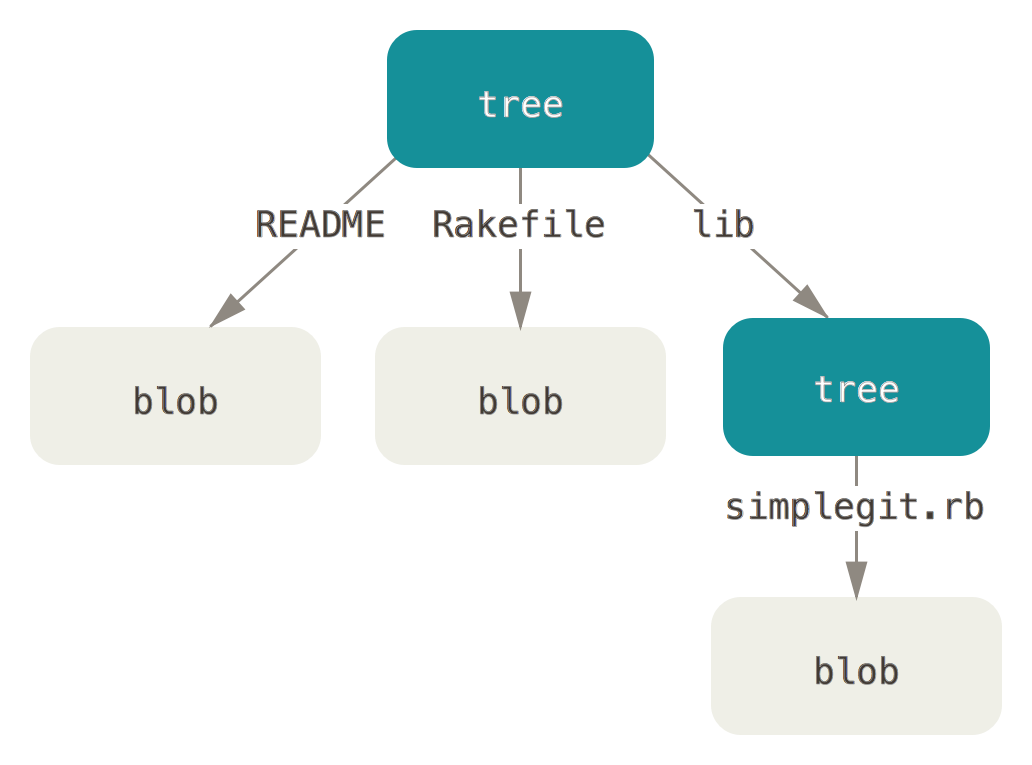
\includegraphics[width=15cm]{technology/data-model-1.png}
            \end{center}
        \end{figure}
        
      You have three trees that specify the different snapshots of your project that you want to track, but the earlier problem remains: you must remember all three SHA-1 values in order to recall the snapshots. You also don’t have any information about who saved the snapshots, when they were saved, or why they were saved. This is the basic information that the commit object stores for you.
      
  
  \section{Pygit2}
    Pygit2 is a set of Python bindings to the libgit2 shared library, libgit2 implements the core of Git. Pygit2 works with Python 2.7, 3.2, 3.3, 3.4 and pypy.
      
    It is likely to work with Python 2.6 and 3.1, but these versions are not officially supported.
    \subsection{libgit2}
      libgit2 is a portable, pure C implementation of the Git core methods provided as a re-entrant linkable library with a solid API, allowing you to write native speed custom Git applications in any language which supports C bindings.
      
      libgit2 is already very usable and is being used in production for many applications including the GitHub.com site, in Plastic SCM and also powering Microsoft's Visual Studio tools for Git. The library provides:
      
      \begin{itemize}
        \item SHA conversions, formatting and shortening
        \item abstracted ODB backend system
        \item commit, tag, tree and blob parsing, editing, and write-back
        \item tree traversal
        \item revision walking
        \item index file (staging area) manipulation
        \item reference management (including packed references)
        \item config file management
        \item high level repository management
        \item thread safety and reentrancy
        \item descriptive and detailed error messages
        \item ...and more (over 175 different API calls)
      \end{itemize}